\section{Modelling Results}
The following simulations were completed using the COMSOL multiphysics software package.
COMSOL uses finite element methods to solve the the laplacian electric field partial differential equation.

\subsection{No Grading}
As a baseline for comparison, a bushing with no foils has been constructed and simulated.
The geometry of the model was built as in figure \ref{figure:Geom:Nograde}.
The system is an axialsymmetric 2D model, which takes the central vertical point $r=0$ as the centre of a cylinder.
\begin{figure}[!h]
   \centering
   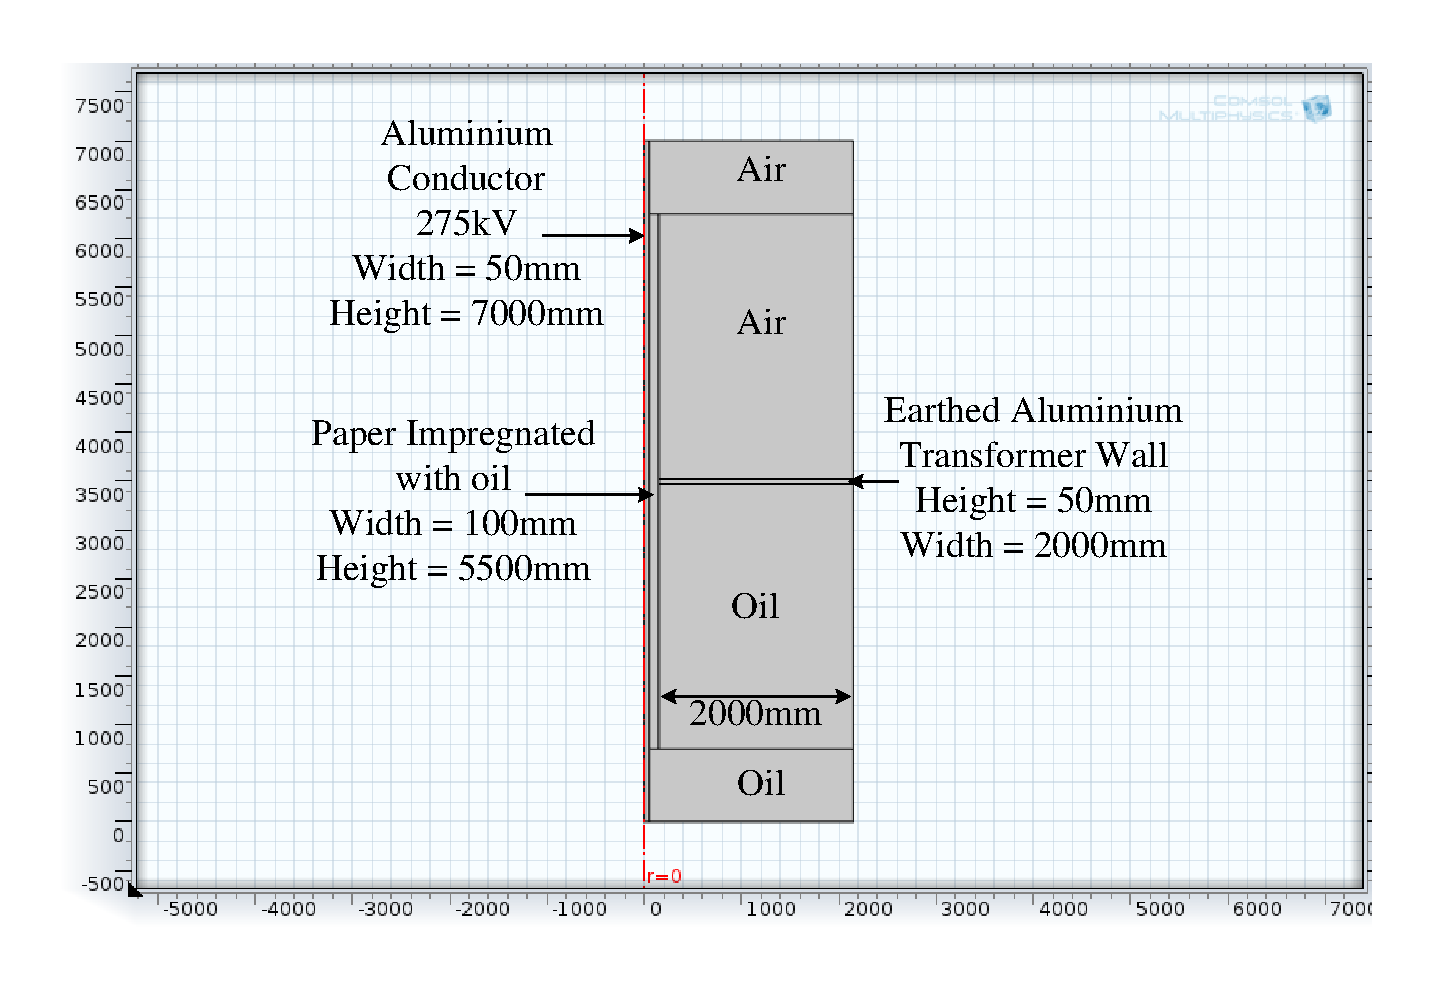
\includegraphics[width = 0.8\textwidth]{NoGradingBlock.pdf}
   \caption{COMSOL Geometry Annotated with Materials - No Grading}
   \label{figure:Geom:Nograde}
\end{figure}

Once the geometry of the model is defined, a finite element mesh can be created as shown in figure \ref{figure:Mesh:Nograde}.
This model is fairly simple, hence a very fine graded mesh was used improving the accuracy of results.
\begin{figure}[!h]
   \centering
   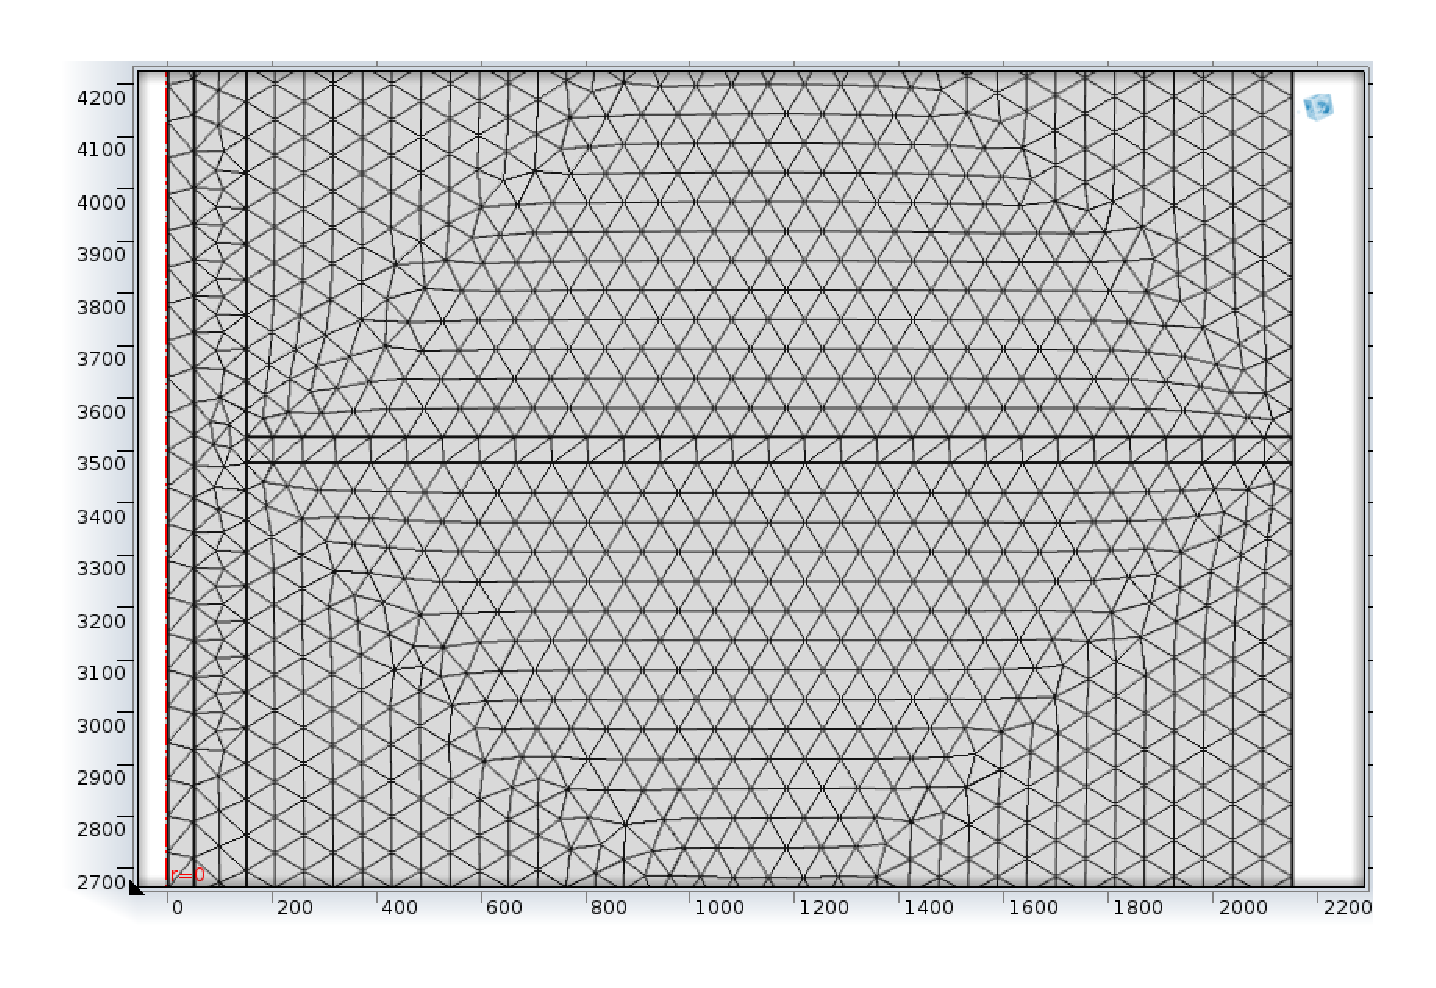
\includegraphics[width = 0.8\textwidth]{NoGradingMesh.pdf}
   \caption{COMSOL Mesh - No Grading}
   \label{figure:Mesh:Nograde}
\end{figure}

The next stage is to define the relative permittivity of each of the materials used for each sub section of the geometry.
The initial conditions must then be set, with the conductor set to 275kV, and the transformer wall and all outer boundaries earthed.
All other boundaries are assumed to be continuity boundaries.

The model can then be solved to give the electric field distribution
\inote{TS - Report done up to here 03/03/2014}
.
\begin{figure}[!h]
   \centering
   \includegraphics[width = 0.8\textwidth]{WideNoGrading.png}
\end{figure}

\begin{figure}[!h]
   \centering
   \includegraphics[width = 0.8\textwidth]{CloseNoGrading.png}
\end{figure}

\begin{figure}[!h]
   \centering
   \includegraphics[width = 0.8\textwidth]{SurfaceGraded21.png}
\end{figure}

\begin{figure}[!h]
   \centering
   \includegraphics[width = 0.8\textwidth]{WideGraded21.png}
\end{figure}

\begin{figure}[!h]
   \centering
   \includegraphics[width = 0.8\textwidth]{CloseGraded21.png}
\end{figure}

\begin{figure}[!h]
   \centering
   \includegraphics[width = 0.8\textwidth]{SurfaceGradedCloseish21.png}
\end{figure}